\section{System Architecture}
\label{sec:arch}

Put some text here to introduce the section...

You can use references such as \ref{sec:arch:control} to refer to a section (in this case, a subsection).


\subsection{Control Interface}
\label{sec:arch:control}

Subsection text here...

\subsubsection{Establishing an Application Link}

You can even have a sub-subsection text here...

And you can reference figures as well, such as Figure~\ref{fig:yancarch} (in this case, the yanc architecture as an example).

\begin{figure}[h]
    \centering
    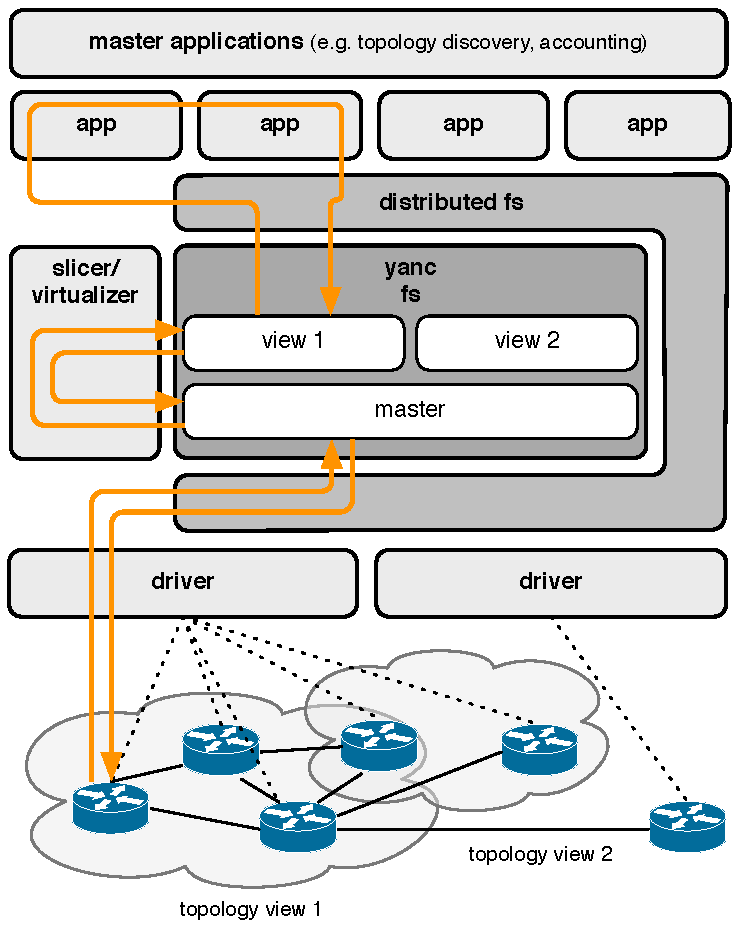
\includegraphics[width=0.85\columnwidth]{figs/yancarch.pdf}
    \caption{Some Figure}
    \label{fig:yancarch}
\end{figure}

